\documentclass[12pt,twoside]{article}
\usepackage[letterpaper, textwidth=6.5in, textheight=9in]{geometry}
\usepackage{amsmath}
\usepackage{hyperref}
\usepackage{graphicx}

\newcommand{\ve}[1]{\ensuremath{\mathbf{#1}}}


\date{\today}
\title{Notes on Computer Hardware \\and Advanced Architectures}
\author{Rachel Slaybaugh}
%-----------------------------------------------------------
%-----------------------------------------------------------
\begin{document}
\maketitle

\section*{General Memory}
Taken from \href{http://thehackerwithin.github.io/berkeley/images/2015.03.18-architecture.pdf}{http://thehackerwithin.github.io/berkeley/images/2015.03.18-architecture.pdf} and some from wikipedia.

\begin{figure}[!ht]
\begin{center}
  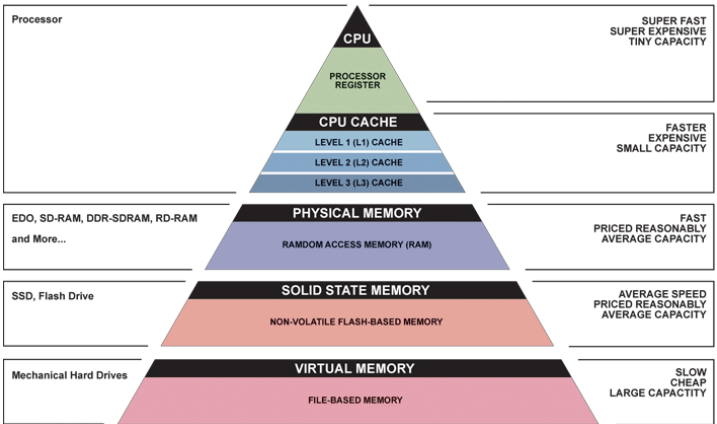
\includegraphics[width=0.8\textwidth, height=0.45\textheight]{cpu-memory-hierarchy}
  \label{fig:cpu-memory}
\end{center}
\end{figure}

Code structure: code is compiled into an assembly program (.s). An assembler turns this into an object, a machine language module (.o). A linker links these and other libraries together into an executable, which is a machine language program (.ext). A loader puts this into memory for execution.

Assembly operands are registers: limited \# of special locations built directly into the hardware (very fast). The MIPS instructions are 32 bits. 

Memory Allocation: \textit{program} (doesn't change size) $\rightarrow$ \textit{static}, variables declared once per program (doesn't change size) $\rightarrow$ \textit{heap}, explicitly created space using e.g.\ malloc $\rightarrow$ \textit{stack}, space for local variables, saved procedure info, etc. (there's a stack pointer that says where this stops.

Once everything is compiled, the machine instructions get translated into memory locations, and switches fire to combine trues and falses (high/low voltage) to make things actually happen.

In execution, 
\begin{enumerate}
  \item We get the 32-bit instruction word from memory; also increment the program pointer to point to the next instruction. 
  \item Decode the instructions and read the data in the correct registers.  
  \item the Arithmetic-Logic Unit (ALU) does instructions
  \item Then load and store instructions happen and in the cache
  \item results of some computation are usually put into a register.
\end{enumerate}

\textbf{Pipelining Hazards}:
\begin{itemize}
  \item structural hazard: a required resource is busy (e.g.\ needed in multiple stages) 
  \item data hazard: data dependency between instructions; need to wait for previous instruction to complete its data read/write
  \item control hazard: flow of execution depends on previous instruction
\end{itemize}

There are XMM registers that are 128 bits each. They take Streaming SIMD Extensions (SSE), an instruction set that works on these in parallel (fetch one instruction, do the work of multiple instructions). Looks like it takes x things (x/2 sets of 2) and does the same operation on each set. 16 x 8 bits or 8 x 16 bit operands.

Layout: 
\begin{itemize}
  \item processor holds data in register file ($\sim$100 Bytes); registers accessed on nanosecond timescale
  \item ``main" memory has more capacity ($\sim$Gbytes); access is $\sim$50-100 ns; hundreds of clock cycles per memory access
  \item disk has \textit{huge} capacity; very slow $\sim$ ms
\end{itemize}	

\textbf{Memory cache} need comes from mismatch between processor and memory speeds. 
It's faster but more expensive than DRAM memory.
It's a copy of a subset of main memory; most processors have separate caches for instructions and data.
In a \textit{direct-mapped} cache, each memory address is associated with one possible block (unit of transfer between cache and memory) within the cache.

Cache misses (failed attempt to read or write a piece of data, resulting in going to main memory): 
\begin{itemize}
  \item compulsory/cold: when a program tries to use something that the program has never requested before. Prefetching and larger cache block sizes can help, though this increases the miss penalty and very large blocks can increase the miss rate.
  \item capacity: cache cannot contain all blocks accessed by the program. Increase cache size, which may increase access time. 
  \item conflict/collision: multiple memory locations mapped to the same cache location. Can increase cache size; increase associativety (may increase access time). 
\end{itemize}

\section*{GPU Memory Overview}
\href{http://gpgpu.org/static/sc2006/slides/03.owens.memoryModelOverview.pdf}{http://gpgpu.org/static/sc2006/slides/03.owens.memoryModelOverview.pdf}


\section*{MICs}
Intel XeonPhi, some background
\begin{itemize}
\item CMOS\textemdash complementary metal oxide semiconductor\textemdash is a technology for constructing integrated circuits. Is used in microprocessors, among others. Usually pairs of p-type and n-type metal oxide semiconductor field effect transistors for logic functions. Use low power and have high noise immunity; less waste heat. Enables high density of logic functions on a chip. \href{https://en.wikipedia.org/wiki/CMOS}{https://en.wikipedia.org/wiki/CMOS} 2015.12.16.

\item 22 nm (vs.\ 14 nm) process node: typical half-pitch for a memory cell in a CMOS. KNC uses 22 nm and KNL usses 14 nm. I don't understand much about this, but it sounds like how many memory components can fit on a device is controlled / limited by this. \href{https://en.wikipedia.org/wiki/Xeon_Phi}{https://en.wikipedia.org/wiki/Xeon_Phi} 2015.12.17.

\item texture sampling is used to determine the texture color for a texture mapped pixel; this is a type of anti-aliasing \href{https://en.wikipedia.org/wiki/Texture_filtering}{https://en.wikipedia.org/wiki/Texture_filtering} 2015.12.17.

\item Mesh network is a network topology in which each node relays data for the network. All mesh nodes cooperate in the distribution of data in the network. Mesh networks can relay messages using either a flooding technique or a routing technique. With routing, the message is propagated along a path by hopping from node to node until it reaches its destination. To ensure all its paths' availability, the network must allow for continuous connections and must reconfigure itself around broken paths, using self-healing algorithms such as Shortest Path Bridging. \href{https://en.wikipedia.org/wiki/Mesh_networking}{https://en.wikipedia.org/wiki/Mesh_networking} 2015.12.17.

\item Knights Corner uses Intel's Tri-gate technology with more than 50 cores per chip and was Intel's first MIC, released in late 2011/mid 2012. 22nm: Xeon Phi 3100 could do 1 tFLOPS of double precision, 240 GB/s memory bandwidth at 300 W. Xeon Phi 5110P was 1.01 tFLOPS of double precision, 320 GB/s at 225 W. Xeon Phi 7120P was 1.2 tFLOPS and 352 GB/s @ 300 W.

\item Knights Landing 

\end{itemize}

\href{https://software.intel.com/sites/default/files/managed/e9/b5/Knights-Corner-is-your-path-to-Knights-Landing.pdf}{https://software.intel.com/sites/default/files/managed/e9/b5/Knights-Corner-is-your-path-to-Knights-Landing.pdf} 2015.12.16
\begin{itemize}
\item coprocessors require workloads to have concurrency across multiple dimensions - generally not there in supercomputers today.
\item can use OpenMP, MPI, Fortran, TBB, C++
\item need thread scaling, vectorization profitability, and fabric scaling (I don't even know what that is)
\item KNL has better serial code performance, more memory than KNC. KNC requires direct coding for vector intrinsics, KNC has static parameters; KNL has integrated fabric that is better for scaling
\item This ppt had some book and code references near the end
\end{itemize}



\end{document}
